\documentclass[11pt,letterpaper]{article}
\usepackage[utf8]{inputenc}
\usepackage[spanish]{babel} 
\decimalpoint

%----- Configuración del estilo del documento------%
\usepackage{epsfig,graphicx}
\usepackage[left=2cm,right=2cm,top=1.8cm,bottom=2.3cm]{geometry}
\usepackage{fancyhdr}
\usepackage{tikz}
\pagestyle{fancy}
\fancyhf{}
\fancyfoot{}
\graphicspath{{Figuras/}}
\usepackage{hyperref}
\hypersetup{colorlinks=true,linkcolor=blue,citecolor=blue,filecolor=blue,urlcolor=magenta,}

\fancyfoot[RO,LE]{\thepage} % Custom footer text
\fancyheadoffset[RO,LE]{0.01\textwidth}

%------ Paquetes matemáticos básicos --------%
\usepackage{amsmath}
\usepackage{amssymb}
\usepackage{amsthm}

%------ Texto aleatorio ----- %

\usepackage{lipsum}


\usepackage[bibstyle = trad-abbrv,
citestyle = numeric-comp,
backend = bibtex, 
sorting = none, % Sort as they appear
backref=false]{biblatex} %style = trad-abbrv 
\AtEveryBibitem{\clearfield{urldate}}
\AtEveryBibitem{\clearfield{url}}
\AtEveryBibitem{\clearfield{isbn}}
\AtEveryBibitem{\clearfield{month}}
\AtEveryBibitem{\clearfield{day}}
\AtEveryBibitem{\clearfield{issn}}
\AtEveryBibitem{\clearfield{serie}}
\DeclareFieldFormat[article]{volume}{\mkbibbold{#1}}
\addbibresource{Tesis.bib}


\begin{document}
	
	%------ Encabezado -------- %
	
	\begin{center}
		\begin{minipage}{3cm}
			\begin{center}
				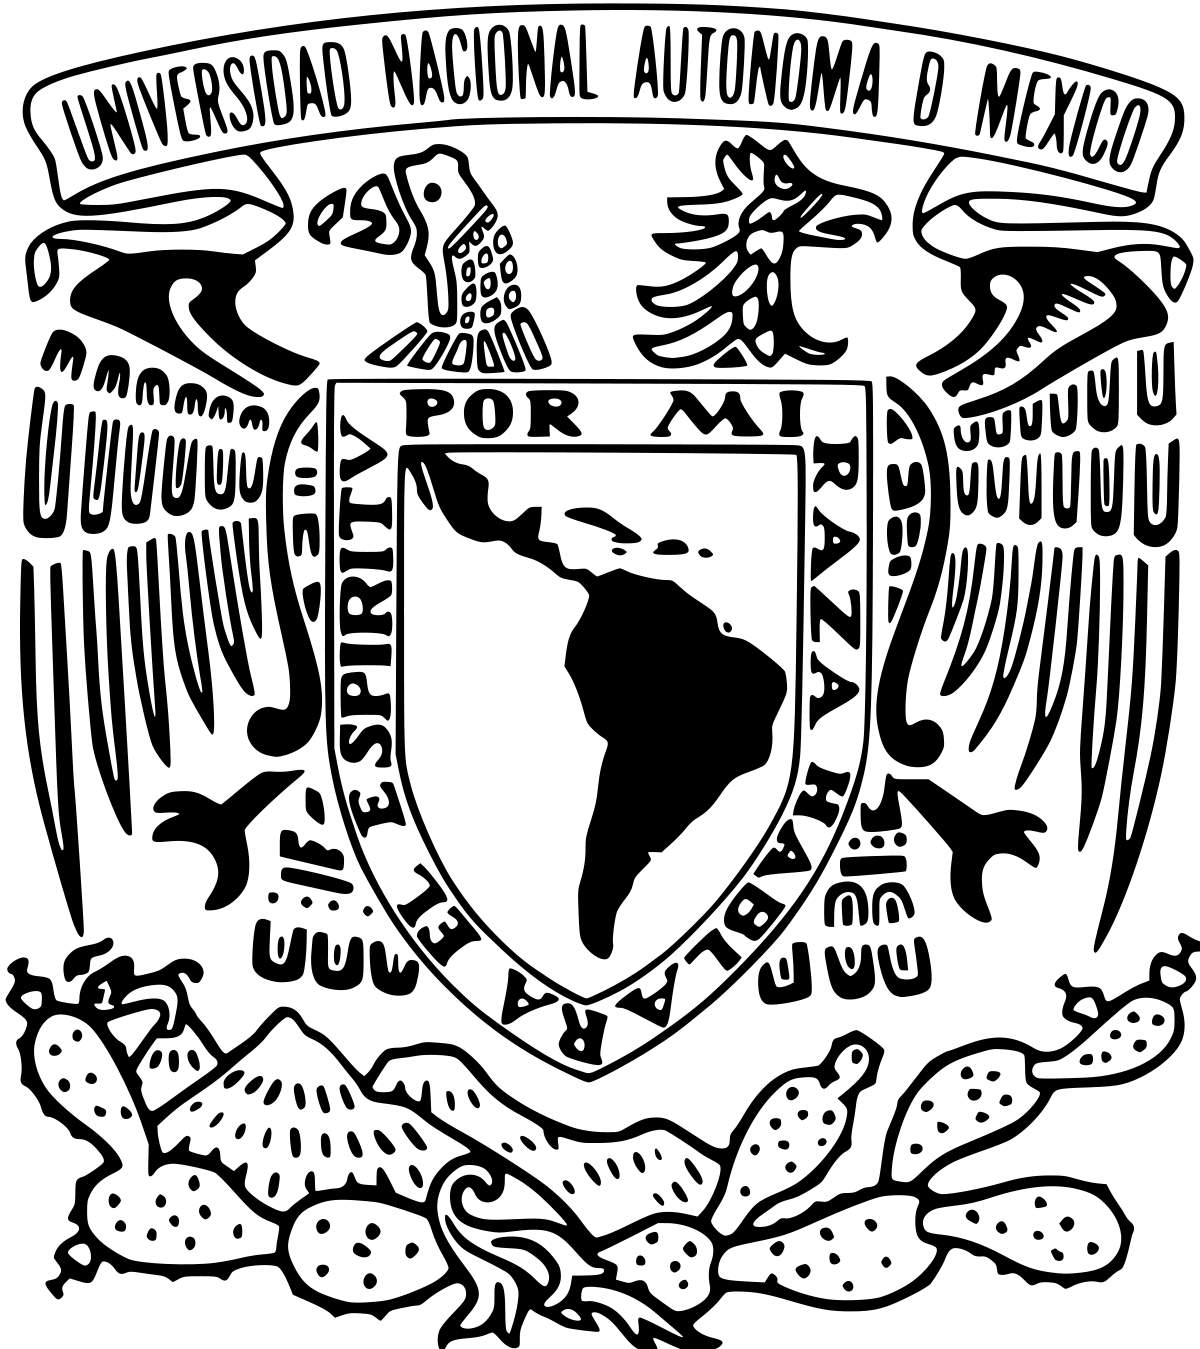
\includegraphics[height=3.4cm]{Logo_UNAM (1)}
			\end{center}
		\end{minipage}\hfill
		\begin{minipage}{3cm}
			\begin{center}
				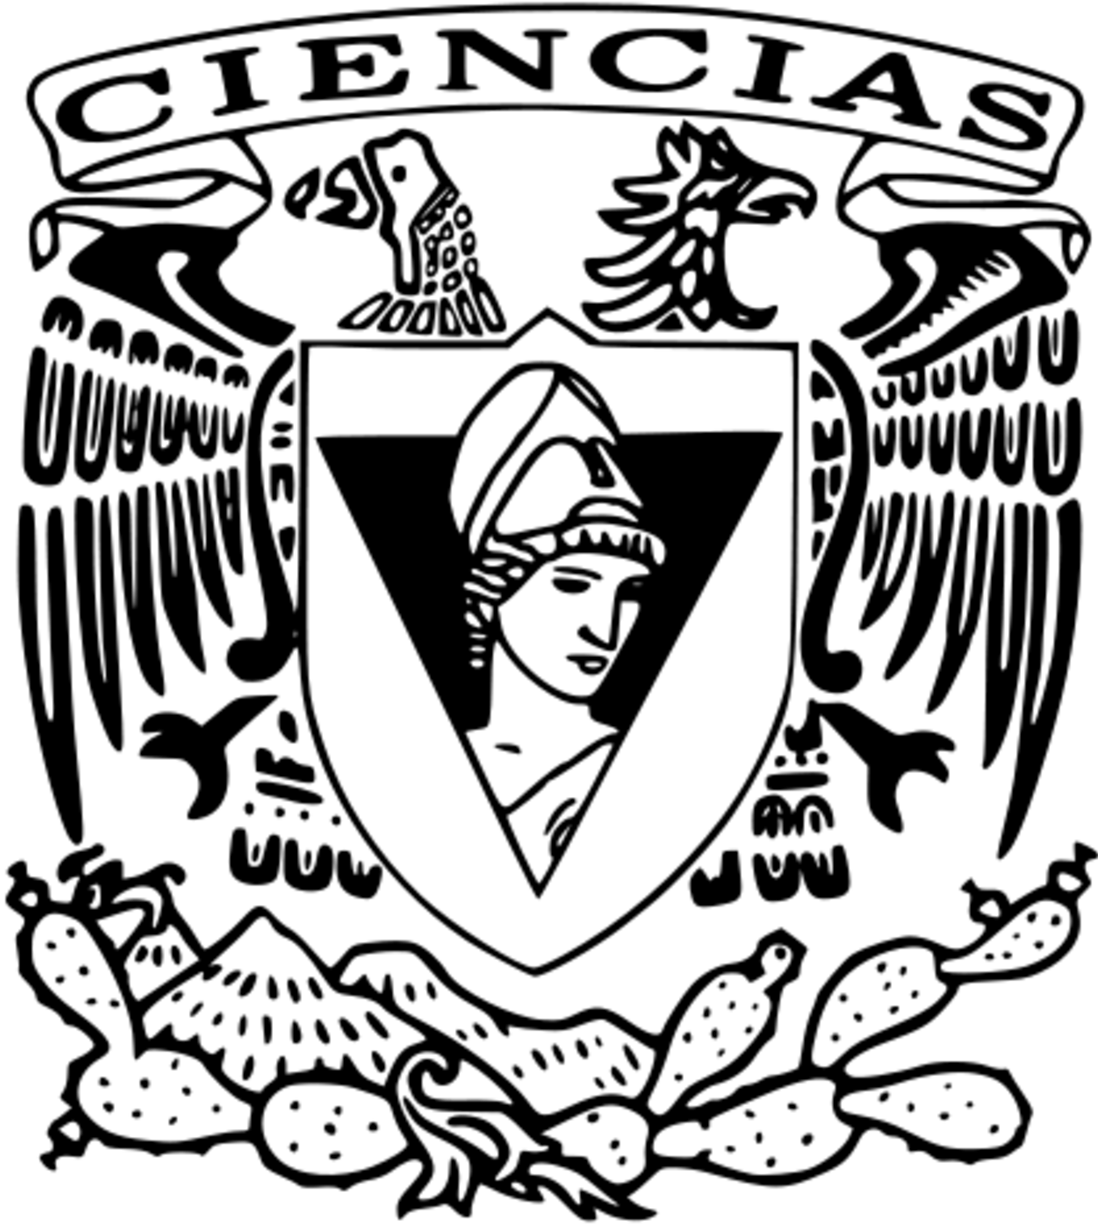
\includegraphics[height=3.4cm]{Logo_FC (1)}
			\end{center}
		\end{minipage}
	\end{center}
	
	\rule{17cm}{0.1mm}
	
	%------ Fin de encabezado -------- %
	\vspace{0.5cm}
	
	\hspace{10cm}{\raggedleft Ciudad Universitaria, 22 de abril de 2025}
	
	\hspace{1cm}
	
	\vspace{0.5cm}
	
	\textsc{Universidad Nacional Autónoma de México}
	
	\textsc{Facultad de Ciencias
	}
	
	\textsc{Coordinación de Física Biomédica
	}
	
	\textsc{Comité Académico de Titulación
	}
	
	\textsc{PRESENTE}\\
	
	\noindent
	% 
	Por medio de la presente, comunico a ustedes el plan de actividades de la alumna Dana Larissa Luna González, con número de cuenta 421122680, para  iniciar el trámite de titulación en la modalidad de tesis. La alumna desarrollará el proyecto titulado ``Cálculo numérico de propiedades ópticas de eritrocitos sanos y enfermos'' bajo mi asesoría, en el grupo de Nanoplasmónica, adscrito al Departamento de Física, Facultad de Ciencias, UNAM.\\
	
	El estudio de las propiedades ópticas de las células biológicas como los osteoblastos \cite{antunesOpticalPropertiesBone2019}, los linfocitos~\cite{yoonIdentificationNonactivatedLymphocytes2017}, y los eritrocitos \cite{bosschaartLiteratureReviewNovel2014}, es de importancia para el área médica por sus potenciales aplicaciones en el diagnóstico y la detección temprana de enfermedades.  En particular, se ha reportado que los eritrocitos presentan alteraciones en su composición y morfología ante diversas formas de anemia \cite{bosschaartLiteratureReviewNovel2014}, lo que afecta directamente su respuesta óptica. Dado que estas células constituyen los principales moduladores de la respuesta óptica de la sangre \cite{bosschaartLiteratureReviewNovel2014}, su estudio resulta fundamental para comprender la interacción luz-tejido en contextos fisiológicos y patológicos.\\
	
	La respuesta óptica de los eritrocitos se modifica por factores como el hematocrito, la concentración de hemoglobina y el nivel de saturación de oxígeno, los cuales afectan sus mecanismos de absorción y esparcimiento de la luz \cite{bosschaartLiteratureReviewNovel2014}, al modificar tanto su función dieléctrica como su morfología celular. En este contexto, el objetivo de la presente tesis de licenciatura es caracterizar las propiedades ópticas de eritrocitos tanto sanos como enfermos, considerando variaciones en su función dieléctrica y morfología. Para ello, se propone cuantificar la respuesta espectral de los eritrocitos mediante el cálculo de las secciones transversales de extinción, esparcimiento y absorción, empleando el método de elemento finito (FEM, por sus siglas en inglés) y comparar los resultados obtenidos con los reportados en la literatura, derivados de otras metodologías \cite{ergulComputationalStudyScattering2010,wriedtLightScatteringSingle2006}.\\
	
	Durante el desarrollo del trabajo, la alumna abordará tres ejes temáticos principales: temas de interés médico sobre eritrocitos,  teorías analíticas de esparcimiento de luz y métodos numéricos para resolver la ecuación de Helmholtz. En el primer apartado se estudiarán las patologías más comunes que afectan a los eritrocitos. En el segundo, se estudiará la solución analítica proporcionada por la teoría de Mie, así como la implementación de las relaciones de Kramers-Kronig \cite{lucariniKramersKronigRelationsOptical2005} para determinar la respuesta espectral de los eritrocitos considerados. Finalmente, se empleará el método de elemento finito a través del software comercial COMSOL Multiphysics y se realizará la construcción de diversas geometrías celulares mediante el software SolidWorks. Ambos programas, cuyas licencias ya están en uso por el grupo de Nanoplasmónica, permitirán simular distintos escenarios patológicos mediante la variación de la función dieléctrica y la morfología celular.\\
	
	Con base en las etapas mencionadas, se propone el siguiente cronograma de actividades:
	
	\begin{itemize} 
		\item \textbf{Abril – mayo:} Revisión de la literatura sobre las propiedades ópticas de eritrocitos sanos y enfermos, así como la clasificación de sus principales alteraciones morfológicas y fisiológicas.
		\item \textbf{Junio – julio:} Estudio del método de elemento finito y familiarización con los programas COMSOL Multiphysics y SolidWorks. Paralelamente, se iniciará la redacción de los capítulos introductorios de la tesis escrita.
		
		\item \textbf{Agosto – septiembre:} Validación del modelo numérico mediante su comparación con casos analíticos conocidos, como la teoría de Mie. Además, se emplearán las relaciones de Kramers-Kronig para determinar la respuesta espectral de los eritrocitos. 
		
		\item \textbf{Septiembre – octubre:} Cálculo de las secciones transversales de absorción, extinción y esparcimiento para eritrocitos sanos y para al menos dos casos de eritrocitos patológicos. Análisis y contraste de los resultados obtenidos.
		
		\item \textbf{Octubre – diciembre:} Redacción del análisis de resultados y de las conclusiones finales de la tesis escrita.
	\end{itemize}
	

	Para el trabajo escrito, se propone el siguiente índice:
	\begin{itemize}
		\item  Agradecimientos
		\item  Resumen
		\item  Introducción: Justificación y antecedentes del trabajo
		\begin{enumerate}
			\item Esparcimiento de ondas electromagnéticas
			\begin{enumerate}
				\item Fundamentos
				\item Método de elemento finito
				\item Relaciones de Kramers-Kronig
			\end{enumerate}
			\item Eritrocitos y sus patologías
			\begin{enumerate}
				\item Funciones dieléctricas
			\end{enumerate}
			\item Resultados
			\begin{enumerate}
				\item Convergencia numérica
				\item Comparación del método analítico y el método numérico
				\item Propiedades ópticas de un eritrocito sano
				\item  Contraste de las propiedades ópticas de eritrocitos sanos con eritrocitos enfermos
			\end{enumerate}
			\item Conclusiones
			\item Trabajo a futuro	
		\end{enumerate}
		\item Apéndice		
	\end{itemize}
	%
	\newpage
	%
	Atentamente,
	
	\vspace{1cm}
	{\hspace{0.7cm}\begin{tabular}{c}
		
\includegraphics[height=2.3cm]{firma}\\[-0.5cm] % Ajusta altura y espacio vertical aquí
		\rule{5.5cm}{0.4pt} \\[0.2cm]
		\textbf{Dana Larissa Luna González} \\
		Estudiante de Física Biomédica \\
		No. de cuenta: 421122680 \\
		Tel.: 776 101 4262 \\
		dana.larissalg@ciencias.unam.mx \\
	\end{tabular}}

	{\vspace{-3.05cm}\hspace{7.5cm}\begin{tabular} { c}
		\rule{5.5cm}{0.4pt} \\[0.2cm]
		\textbf{Dr. Alejandro Reyes Coronado} \\
		Profesor Titular C de Tiempo Completo \\
		Departamento de Física, Facultad de Ciencias, UNAM \\
		Tel.: (55) 5622 4968 \\
		coronado@ciencias.unam.mx \\
	\end{tabular}
	
	
	
	
	
	
	
	
	
	
	
	
	
	
	
	
	
	
	
	
	
	
	
	
	
	
	
	
	
	%%----------------------------------------
	\printbibliography
	
\end{document}



